\documentclass[12pt]{article}

\usepackage{sbc-template}
\usepackage{array}
\usepackage{graphicx,url}
\usepackage[tight,footnotesize]{subfigure}
\usepackage{enumerate}
%encoding
%--------------------------------------
\usepackage[utf8]{inputenc}
\usepackage[T1]{fontenc}
%--------------------------------------
 
%Portuguese-specific commands
%--------------------------------------
\usepackage[portuguese]{babel}
%--------------------------------------


%\usepackage[brazil]{babel}   
%\usepackage[latin1]{inputenc}  
\usepackage[export]{adjustbox}
%fontes personalizadas
\usepackage{enumerate}
\usepackage{bm}
%bibliotecas matem\'{a}ticas
\usepackage{amsmath}
\usepackage{amsfonts}
\usepackage{amssymb}
\usepackage{float}
\usepackage{pst-func}
\usepackage{pst-math}

\usepackage{color, colortbl}
\definecolor{Gray}{gray}{0.95}
\usepackage{kpfonts}
\usepackage[T1]{fontenc}

\usepackage{graphicx,url}

\usepackage{listings}
\definecolor{light-gray}{gray}{0.9}
\lstset{extendedchars=\true,
		inputencoding=ansinew,
		showspaces=false,
		showstringspaces=false,
		showtabs=false,
		tabsize=2,
		backgroundcolor=\color{light-gray}}
     
\sloppy

\title{Análise de Medidas de Centralidade Aplicadas as Redes Ópticas de Telecomunicações}

\author{Silvana Trindade\inst{1}, Guilherme Bizzani\inst{1}, Rodrigo Levinsk\inst{1}, Watson V. C. Junior\inst{1}}


\address{Universidade Federal da Fronteira Sul (UFFS)\\Chapecó,SC-Brasil
  \email{\{syletri,gaioleroo,rd.levinsk,watsonmaster\}@gmail.com}
}

\begin{document} 

\maketitle

\begin{abstract}
 
\end{abstract}
%contextualiza?o
%gap
%proposito
%metodologia
%resultados
%conclusão
\begin{resumo} 

A partir de um conjunto de redes ópticas de telecomunicações, foi realizado uma análise referente as características relevantes para as  medidas de centralidade de grau, de intermediação, de eficiência, de proximidade e, relativa .
As medidas de centralidade buscam obter vértices relevantes em função de algumas invariantes do grafo, podendo  influenciar diretamente na implantação de uma rede.
Os resultados experimentais evidenciaram que a centralidade de proximidade é influenciada pelo grau médio; a centralidade de intermediação pelo número de ligações e nós; a centralidade de eficiência pelo grau médio.
\end{resumo}


\section{Introdução}
%contextualização
%gap
%metodo proposto
As redes de telecomunicações envolvem uma série de cálculos e análises prévias para sua eficiente implantação, prevenindo sobrecargas e garantindo sua integridade.
Em \cite{pavan} são apresentadas algumas características para as topologias físicas de redes reais devem respeitar alguns pré requisitos, entre eles estão: o grafo que representa a topologia deve ser  2-conexo, o grau minimo de cada nó deve ser dois e devem existir no mínimo dois caminhos disjuntos de um nó de origem até um de destino.

A análise da confiabilidade de rede e a identificação de seus principais elementos são importantes ferramentas para diversos estudos práticos, como por exemplo, a expansão e manutenção de sistemas elétricos, de transportes e de telecomunicações \cite{silva}.
Em \cite{pavan} são identificadas características relevantes de topologias sobreviventes a partir de um conjunto de $29$ topologias físicas de redes reais, como o número médio de saltos, coeficiente de proteção, e coeficiente de restauro.

O método proposto faz um estudo de cinco medidas de centralidade em redes ópticas de telecomunicações aplicadas a um conjunto de 9 à 100 nós.
Utilizamos um conjunto de $12$ redes de referência que apresentam características semelhantes, com o intuito de melhor avaliar a relevância dos nós para cada medida.

Em \cite{Brandes01afaster} é apresentado um algoritmo para obter a centralidade de intermediação do grafo com complexidade  $O(n^2 log n+nm)$, sendo $m$ o número de ligações e $n$ o número de nós.
Além disso, com o mesmo obtivemos as outras medidas de centralidade, necessitando somente de algumas estruturas a nível de linguagem.

O presente artigo esta organizado da seguinte forma: na Seção \ref{sec:mc} é apresentado o conceito das cinco medidas de centralidade utilizadas.
Posteriormente na  Seção \ref{sec:met} será abordado o método utilizado. 
Na Seção \ref{sec:result} são apresentados os resultados.
E finalmente na Seção \ref{sec:conc} as conclusões e trabalhos futuros serão expostos. 




\section{Medidas de Centralidade}\label{sec:mc}

O estudo de redes é de grande interesse na área científica, dada a capacidade de uma rede poder representar por meio de modelagem diversos problemas de natureza real.
Em grafos como modelos para redes, as medidas de centralidade buscam medir a variação da relevância dos vértices, em função de alguns invariantes do grafo \cite{freitas}.

Em \cite{freitas} intuitivamente, em uma rede, os nós mais centrais são aqueles que a partir dos quais podemos atingir qualquer outro com mais facilidade ou rapidez. Buscamos com este trabalho direcionar as medidas para redes de telecomunicações as quais são influenciadas por $n$ variáveis, grau, número de ligações, número de nós, dentre outras.




\subsection{Centralidade de Eficiência}
Em  Pesquisa  Operacional,  alguns  problemas  de  localização  consistem  em  se determinar um local de modo que minimize o tempo máximo de viagem entre o mesmo e todas as demais localizações.Estes problemas possuem diversas aplicações práticas, como  por  exemplo,  a  instalação  de  um  hospital,  cujo objetivo  é  minimizar  o  tempo máximo de atendimento de uma ambulância a uma possível emergência\cite{freitas}.

Com o intuito de resolver este tipo de problemas foi que, em 1995,  HAGE e HARARY propuseram a medida de {\it Centralidades de eficiência} que baseia-se no conceito de excentricidade de um vértice e pode ser definida como: 

Seja  {\it G} um grafo conexo com {\it n} vértices  e seja $v_k$ um vértice de {\it G}, a {\it centralidade de eficiência} de $v_k$ é dada pelo inverso da excentricidade de $v_k$, ou seja,
\begin{center}
\begin{equation}
C_{eff}(v_k)= \frac{1}{e_{(v_k)}},\label{ce}
\end{equation}
\end{center}
O algoritmo desenvolvido apresenta os seguintes passos:
\begin{enumerate}
\item Buscar o maior número de saltos do vértice quanto a todos ou outros, utilizando a matriz de caminhos mínimos previamente calculada com auxílio do algoritmo de \cite{Brandes01afaster}.
\item Calcula-se a centralidade de eficiência (\ref{ce}) para cada vértice. 
\item Armazena-se o maior valor atual da centralidade de eficiência.
\item Obtém-se o valor da centralidade de eficiência e todos os vértices que resultam neste valor. 
\end{enumerate} 
   
   
   
   
\subsection{Centralidade de Grau e Centralidade Relativa}
Na Centralidade de Grau, o vértice com gau maior é considerado o  mais central.
Segundo \cite{freitas} a equação obtida pelo somatório onde o grau do vértice $d_{k}$ é constuido pela soma da matriz de adjacência $a_{kj}$.
\begin{center}
\begin{equation}
d_{k}= \sum_{j=1}^{n}a_{kj}
\end{equation}
\end{center}

Na Centralidade Relativa é usada a proporção do valor do grau em relação do tamanho do grafo, dada por:
\begin{center}
\begin{equation}
{c}'_{d}(v_{k})=\frac{d_k}{n-1}.
\end{equation}
\end{center}

O algorítimo de obtenção da centralidade de grau realiza os seguintes passos:
\begin{enumerate}
\item Considera o grau máximo como zero.
\item Compara os graus dos vértices.
\item Caso o valor do nó atual seja maior, ele substitui o valor máximo pelo seu valor.
\item Com o valor estabelecido da centralidade de grau, se calcula a centralidade relativa usando o total de nós na rede.
\end{enumerate}





\subsection{Centralidade de Intermediação}
Em \cite{freitas} a centralidade de intermediação foi introduzida com o objetivo de expressar a influência que um vértice sobre seus pares em um grafo.
A medida consiste em obter o número de geodésicas entre todos os pares de vértices do grafo a partir de um determinado vértice \cite{freitas}.

Para calcular a centralidade de intermediação ($C_I$) utiliza-se: 
\begin{center}
\begin{equation}
C_I(v_k)=\sum_{i\neq j \neq v_{k}} \frac{b_{ij}(v_k)}{b_{ij}},
\end{equation}
\end{center}
onde $b_{ij}$ representa o número total de geodésicas entre os vértices $i$ e $j$ e  $b_{ij}(v_k)$ representa o número de geodésicas entre $i$ e $j$ que possuem ao longo do caminho o vértice $(v_k)$.
Sendo o nó com maior centralidade de intermediação será o mais central da rede \cite{ufimtsev} \cite{freeman}.

O algoritmo de \cite{Brandes01afaster} foi utilizou para calcular a centralidade de intermediação, as seguintes etapas:
\begin{enumerate}
\item Obter as geodésicas de $i$ a $j$.
\item Verificar se existe o nó $v_k$ em alguma geodésica de $i$ até $j$.
\item Calcular a centralidade de intermediação para todos os nós.
\end{enumerate}
Onde serão repetidas de $k = 0,1,2,\dots,n$ nós.




\subsection{Centralidade de Proximidade}
A mais simples e natural das medidas de centralidade do vértice baseada na proximidade foi chamada de centralidade de proximidade, e é baseada na soma das distâncias de um  vértice em relação aos demais vértices do grafo\cite{freitas}.

Para calcular a Centralidade de Proximidade usamos a seguinte fórmula:
\begin{center}
\begin{equation}
C_P(v_k)=\frac{1}{\sum\limits_{j = 1}^n dist(v_j,v_k)},
\end{equation}
\end{center}
Sendo {\it G} um grafo conexo com {\it n} vértices e seja $v_k$ um vértice de {\it G}. A centralidade de proximidade de $v_k$ é dada pelo inverso da soma das distâncias de $v_k$ a todos os demais vértices do grafo.
Para realizarmos esta fórmula em nosso algoritmo efetuamos os seguintes passos:
\begin{enumerate}
\item Utiliza-se a matriz de caminhos mínimos criada anteriormente para fazer o cálculo proposto na fórmula anterior e guardar qual o menor valor encontrado.
\item Posteriormente é procurado pelo menor valor, o qual será obtido como resultado final junto com todos os vértices que possuem este valor.
\end{enumerate}

%Metodo proposto ------------------------------------------------------
\section{Método Proposto}\label{sec:met}

Em \cite{Brandes01afaster} é apresentada uma proposta de algoritmo para calcular a centralidade de intermediação de um vértice em um grafo. O mesmo utiliza do método dos caminhos de Dijkstra com a modificação, busca todos os caminhos mínimos ao invés de um único entre um vértice origem $s$ em um de destino $t$.

As medidas de centralidade apresentadas neste artigo utilizam de caminhos mínimos, assim fez-se o uso do algoritmo de \cite{Brandes01afaster} para obter as geodésicas dos grafos que representam as redes de telecomunicações.

\section{Resultados e Discussões}\label{sec:result}
\begin{figure}[htp]
	\centering
	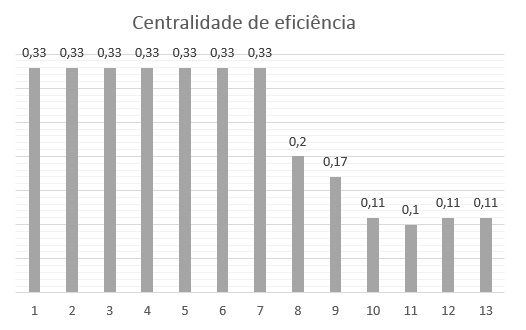
\includegraphics[scale=0.75]{Imagens/Eficiencia}
	\caption{Centralidade de Eficiência}
	\label{fig:fig1}
\end{figure}
Texto
\begin{figure}[htp]
	\centering
	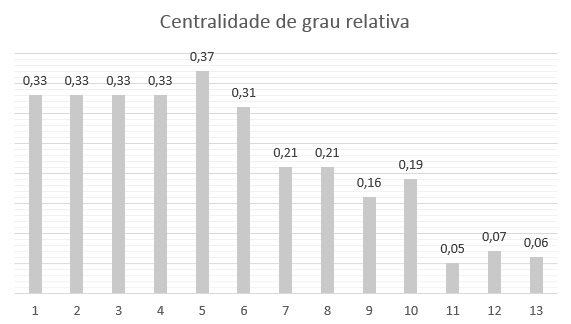
\includegraphics[scale=0.75]{Imagens/GrauRelativa}
	\caption{Centralidade Relativa de Grau}
	\label{fig:fig2}
\end{figure}
Texto
\begin{figure}[htp]
	\centering
	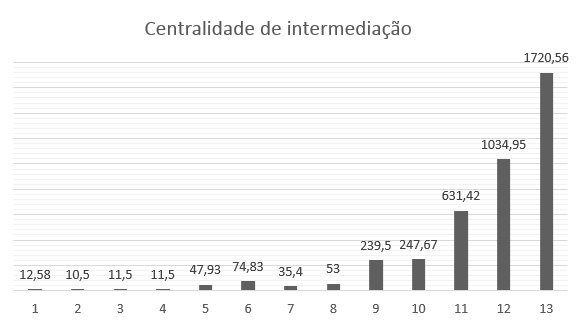
\includegraphics[scale=0.75]{Imagens/Intermediacao}
	\caption{Centralidade de Intermediação}
	\label{fig:fig3}
\end{figure}
Texto
\begin{figure}[htp]
	\centering
	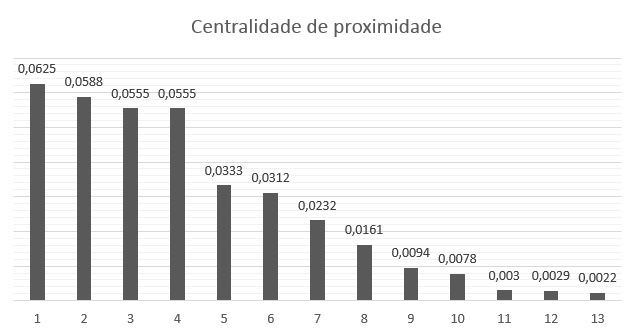
\includegraphics[scale=0.75]{Imagens/proximidade}
	\caption{Centralidade de Proximidade}
	\label{fig:fig4}
\end{figure}
Texto
\begin{figure}[htp]
	\centering
	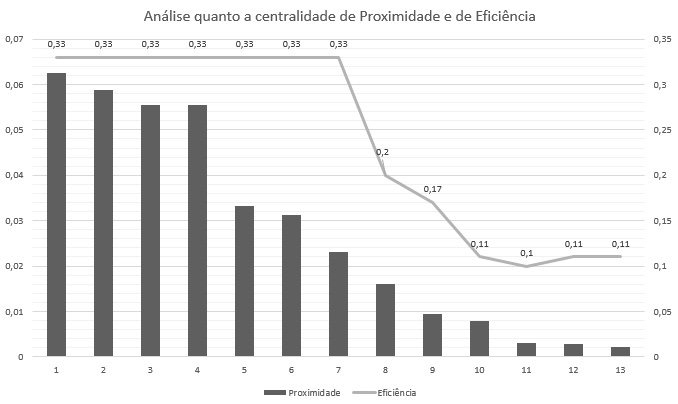
\includegraphics[scale=0.70]{Imagens/ProximidadeEficiencia}
	\caption{Centralidade de Proximidade e Eficiência}
	\label{fig:fig4}
\end{figure}
Texto

A execução deste algoritmo resultou em um conjunto de dados que são apresentados na Tabela \ref{tab:tab1}. 

%como foi feito
%descrever etapas
\begin{table}[htp]
\caption{CONJUNTO DE REDES REAIS DE REFERÊNCIA}\label{tab:tab1}
\centering
\begin{tabular}{cll*{9}{l}r}
\hline\rowcolor{Gray}
Número & Rede & \textit{N} & \textit{L} & $\langle \delta \rangle$ & $C_G$ & $C_R$ & $C_E$ & $C_P$ & $C_I$\\ 
\hline
1   &Abilenecore &10    &13     &2.6    &3   &0.33    &0.33     &0.0625     &12.58\\
2   &RNP        &10     &12     & 2.4   &3   &0.33    &0.33     &0.0588     &10.50\\
3   &Learn      &10     & 11    &2.2    &3   &0.33    &0.33     &0.0555     &11.50\\
4   &Bren       &10     & 11    &2.2    &3   &0.33    &0.33     &0.0555     &11.50\\
5   &Germany    &17     & 26    &3.06   &6   &0.37    &0.33     &0.0333     &47.93\\
6   &Arnes      &17     & 20    &2.35   &5   &0.31    &0.33     &0.0312     &74.83\\
7   &Arpanet    &20     & 32    &3.2    &4   &0.21   &0.33      &0.0232     &35.40\\
8   &Sweden     &20     & 24    &2.4    &4   &0.21   &0.20      &0.0161     &53.00\\
9   &Metrona    &33     & 41    &2.48   &5   &0.16   &0.17      &0.0094     &239.50\\
10  &Loni       &33     & 37    &2.24   & 6  &0.19   &0.11      &0.0078     &247.67\\
11  &Internet2  &56     & 61    &2.18   & 3  &0.05   &0.10      &0.0030     &631.42\\
12  &Coronet    &75     & 97    & 2.59  & 5  &0.07   &0.11      &0.0029     &1034.95\\
13  &Usa        &100    &171    & 3.42  & 6  &0.06    &0.11     &0.0022     &1720.56\\
\hline
\end{tabular}
\end{table}

 A centralidade de intermediação pelo número de ligações e nós, a centralidade de eficiência pelo grau médio.
 
A centralidade de proximidade $C_P$ é diretamente influenciada pelo grau médio da rede $\langle \delta \rangle$, quanto maior o grau médio maior será o valor da centralidade de proximidade em redes com o mesmo número de nós. Esta medida pode ser considerada estável quanto a variações não contendo grandes diferenças entre redes de maior pra menor porte e vice-versa.
\

Da mesma forma, a centralidade de eficiência $C_E$ é influenciada pelo grau médio $\langle \delta \rangle$, porém a centralidade de eficiência sofre menos oscilações pelo grau médio variando de $0>C_E<=0.5$, onde 0.5 é considerada uma eficiência ótima para este conjunto de dados.

Já a centralidade de grau $C_G$ não sofre influência de outras invariantes da rede além do próprio grau do nó. 
A centralidade relativa de grau $C_R$ é influenciada pelo grau máximo e pelo número de vértices, quanto maior o número de ligações da rede maior é a medida.

%exemplo de inserir img
% \begin{figure}[htp]
% \centering
% \includegraphics[width=6in,natwidth=516,natheight=65]{grafico.png}
% \caption{comentarios}
% \label{fig:fig1}
%\end{figure}

%graficos
%analises
\section{Conclusão e Trabalhos Futuros}\label{sec:conc}

\bibliographystyle{sbc}
\bibliography{sbc-template}

\end{document}